\section{Ejercicio 3 - TaskBatch}

Se programó un tipo de tarea llamado {\tt TaskBatch}.  Este tipo de tarea realiza {\it cant_bloqueos} llamadas bloqueantes en momentos elegidos pseudoaleatoriamente, y cada bloqueo dura 1 ciclo.  Además, utiliza el el CPU durante {\it total_cpu} ciclos, incluyendo el tiempo necesario para lanzar las llamadas bloqueantes, pero no el tiempo en el que el proceso permanece bloqueado.

\subsection{Algoritmo}

La idea de nuestro algoritmo se basa en decidir, a cada ciclo y de manera pseudoaleatoria, si se realiza un bloqueo o no.  Para tomar esta decisión vamos a tomar un valor entero ``random'' entre 0 y 1 (1 para bloquear y 0 para no hacerlo), nuevamente utilizando la función {\tt rand()} de C++.

Como cada llamada bloqueante consume 1 ciclo de utilización de CPU, podemos decir que {\it total_cpu} incluye {\it cant_bloqueos} ciclos destinados a las llamadas bloqueantes, y el resto son usos ``puros'' de CPU.  Por este motivo, la decisión pseudoaleatoria de bloquear la tarea se realizará $total\_cpu - cant\_bloqueos$ veces. Una vez realizados todos los usos ``puros'' de CPU, sólo resta realizar las llamadas bloqueantes necesarias para completar {\it cant_bloqueos}.

La Figura \ref{cod-tbatch} muestra el pseudo-códgo de este algoritmo.

\begin{figure}[!htb]
\begin{codebox}
\Procname{$\proc{TaskBatch}(total\_cpu,cant\_bloqueos)$}
\li \For $i \leftarrow 0 .. (total\_cpu - cant\_bloqueos - 1)$
\li \Do 	$bloquear \leftarrow $ valor ``random'' en [0,1]
\li 		\If $bloquear == 1 \wedge $ aún hay bloqueos por hacer
\li 		\Then 	bloquear durante 1 ciclo
\li	 			decrementar $cant\_bloqueos$
\li 		\Else	usar CPU durante 1 ciclo
		\End
	\End
\li \While aún hay bloqueos por hacer
\li \Do 		bloquear durante 1 ciclo
\li 			decrementar $cant\_bloqueos$
	\End
\end{codebox}
\caption{Pseudocódigo TaskBatch}\label{cod-tbatch}
\end{figure}

\subsection{Pruebas}

El lote que utilizamos consta de tres tareas, las mismas tratan de mostrar el comportamiento de nuestra {\tt TaskBatch}.  Las características de estas tareas son las siguientes:

\begin{enumerate}
\item Posee sólo una llamada bloqueante, para mostrar que no siempre realizará la llamada bloqueante al final, sino que la ubicará en el medio con mayor probabilidad.
\item Posee muchas llamadas bloqueantes, de manera de que las mismas se realicen de forma consecutivas al final con mayor probabilidad.
\item Posee un número de llamadas bloqueantes cerca de un tercio de la cantidad de tiempo de cpu, para mostrar que las llamadas bloqueantes no necesariamente siguen un patrón.
\end{enumerate}

La Figura \ref{fig-batch} grafica el lote descrito utilizando un scheduler de tipo FCFS.

\begin{figure}[!htb]
\begin{center}
  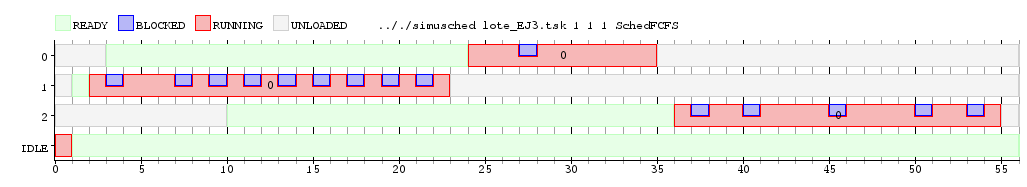
\includegraphics[scale=0.45]{imagenes/ej3.png}
\end{center}
\caption{Simulación para TaskBatch, 1 núcleo, 1 ciclo de cs}\label{fig-batch}
\end{figure}
